\begin{table*}
\begin{center}
    \begin{tabular}{ l l || c c c c c c c}
    \hline
Score norm & Replay env. &  GMM & SGL & SGL-NAP  & SGL-FA & FA & IV & IV-PLDA \\ 

 \hline \hline
& (Baseline) & 9.08 & 7.89 & 6.35 & 6.08 & 5.60 & 6.67 & 3.20\\
No & Office  & 40.26 & 34.43 & 33.52 & 30.72 & 33.85 & 27.83 & 29.11\\
norm & Corridor & 35.71 & 28.24 & 28.53 & 25.75 & 29.92 & 23.02 & 22.78\\
& None & 51.59 & 49.64 & 49.49 & 49.73 & 49.37 & 49.38 & 49.37\\
\hline
& (Baseline) & 8.63 & 8.13 & 6.31 & 5.72 & 5.61 & 6.72 & 2.98\\
With & Office  & 60.32 & 92.98 & 29.92 & 28.54 & 30.12 & 28.89 & 30.30\\
norm & Corridor & 55.91 & 88.20 & 23.59 & 21.62 & 24.97 & 23.31 & 24.53\\
& None & 64.40 & 96.67 & 49.44 & 49.31 & 49.67 & 49.06 & 49.46\\
\hline
    \end{tabular}
    \caption{EER values for different ASV systems for various acoustic environment of replay attacks, with and without score normalisation. }
		\label{tab::results_EER}
   \end{center}
\end{table*}


\begin{figure}
	\centering
	\begin{minipage}{.5\textwidth}
	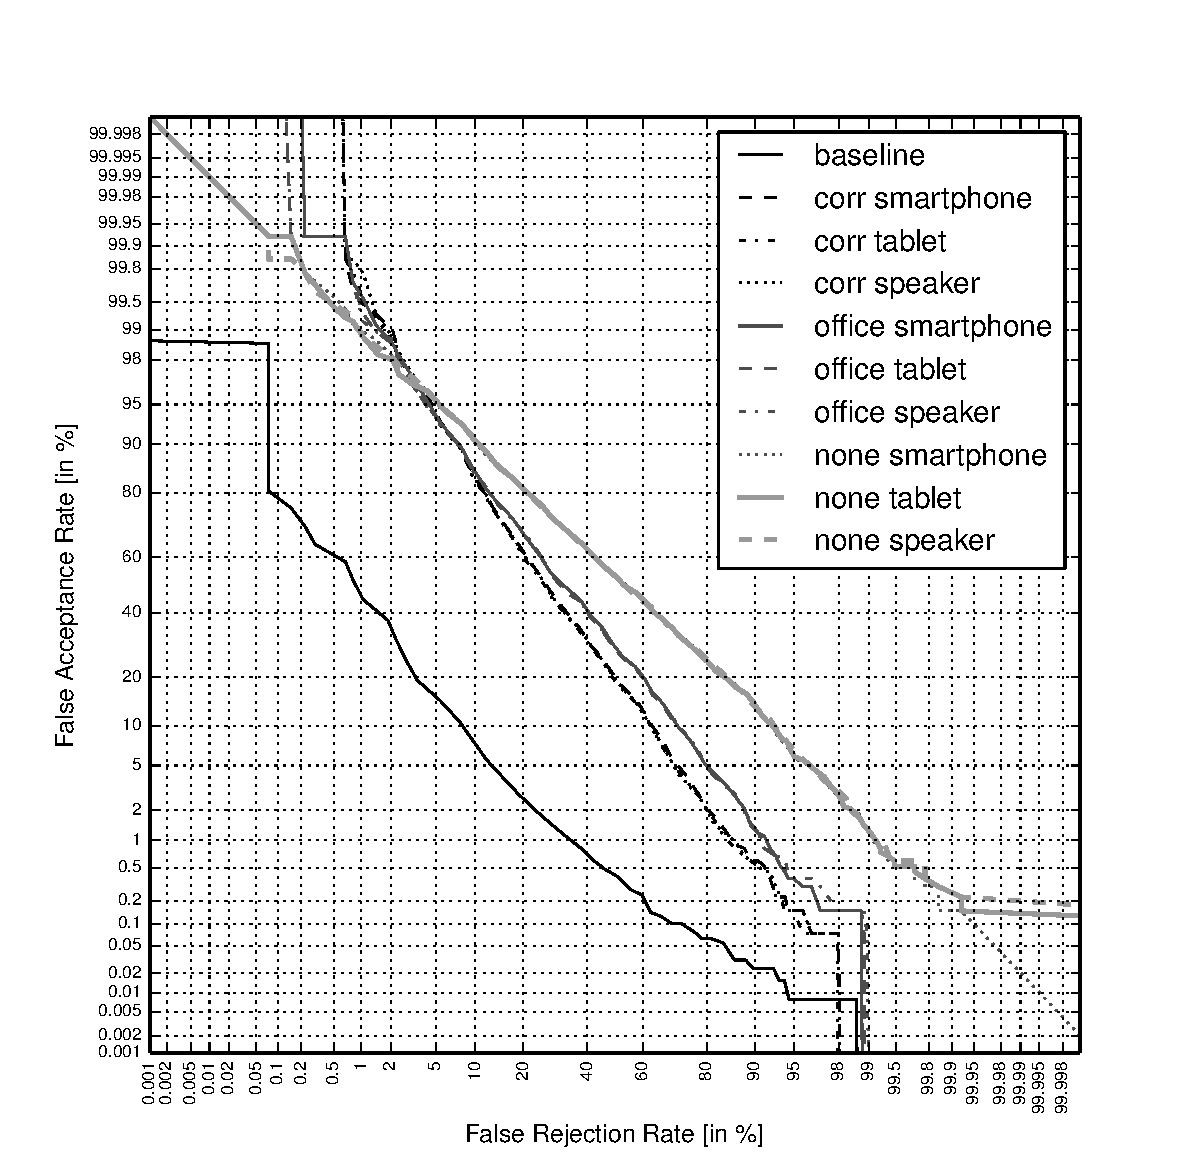
\includegraphics[width=1\linewidth]{Figs/DETs_GMM.pdf}
	\caption{DET plots for the GMM-UBM system for various replay configurations, compared to the baseline performance.}
	\label{fig::DETs_replay_GMM}
	\end{minipage}
	\begin{minipage}{.5\textwidth}
	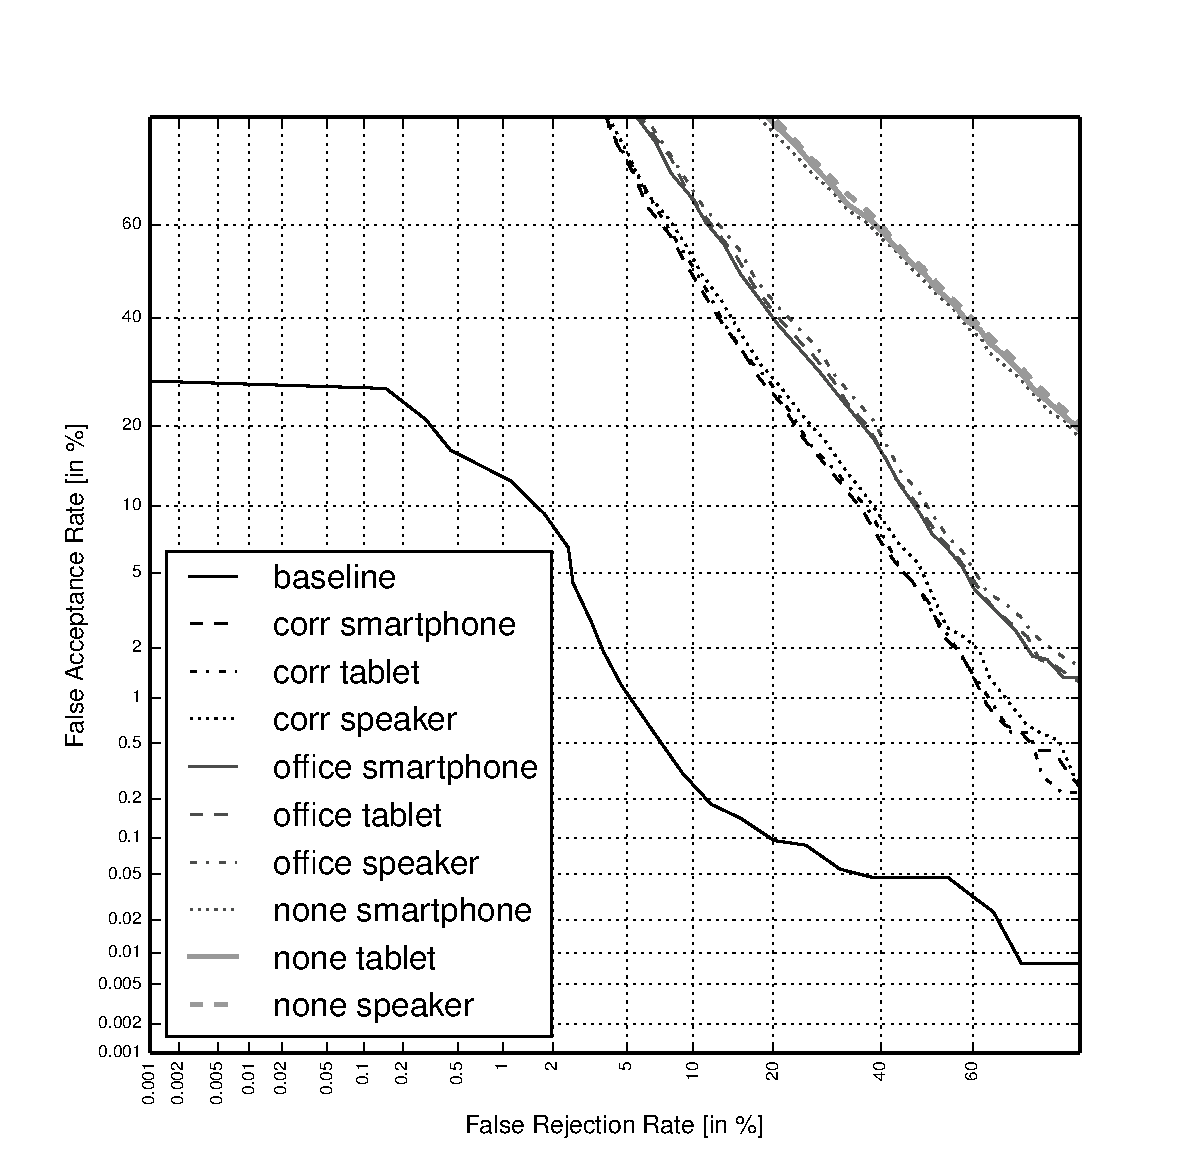
\includegraphics[width=1\linewidth]{Figs/DETs_IV.pdf}
	\caption{DET plots for the IV-PLDA system for various replay configurations, compared to the baseline performance.}
	\label{fig::DETs_replay_IV}
	\end{minipage}


\end{figure}



\begin{figure}
	\centering
	\begin{minipage}{.5\textwidth}
	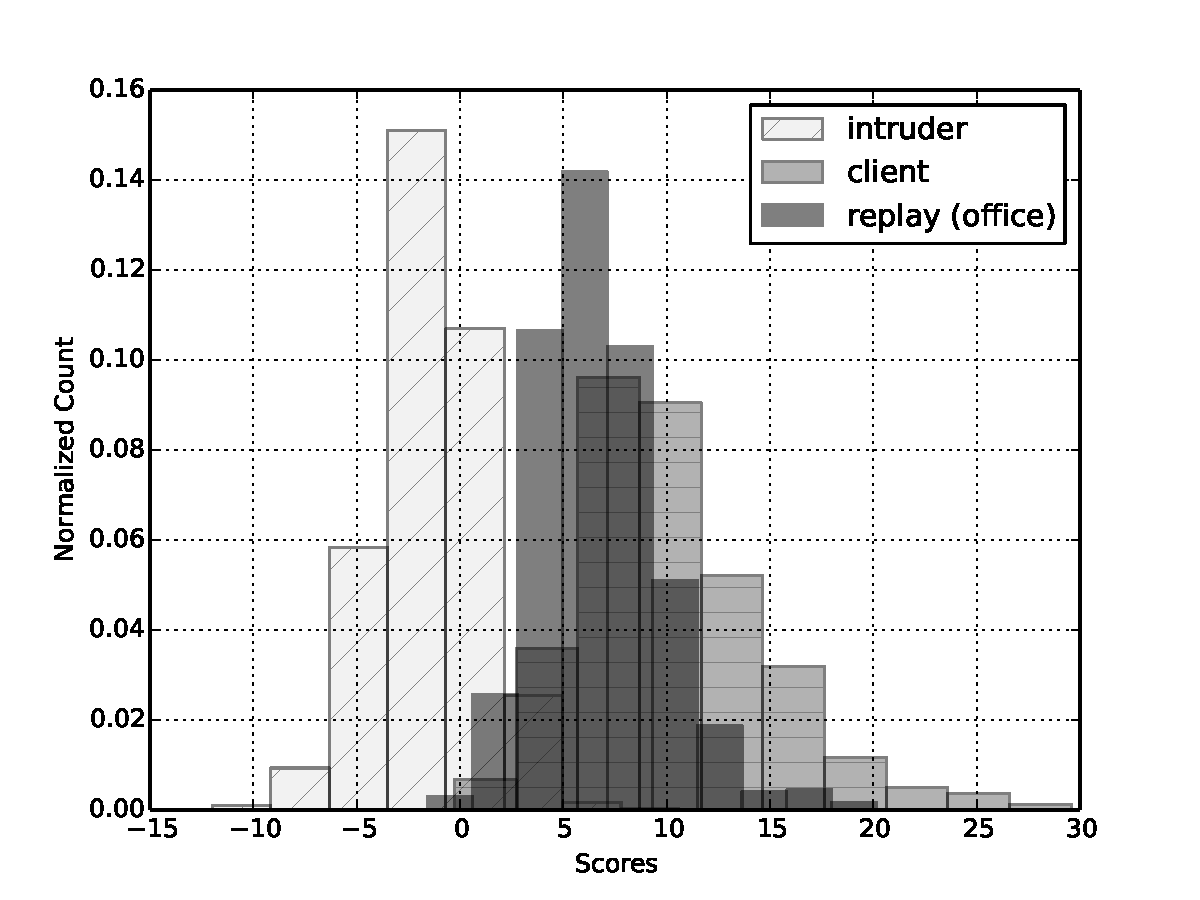
\includegraphics[width=1\linewidth]{Figs/dist_IV_off.pdf}
	\end{minipage}

%	\begin{minipage}{0.5\textwidth}
%	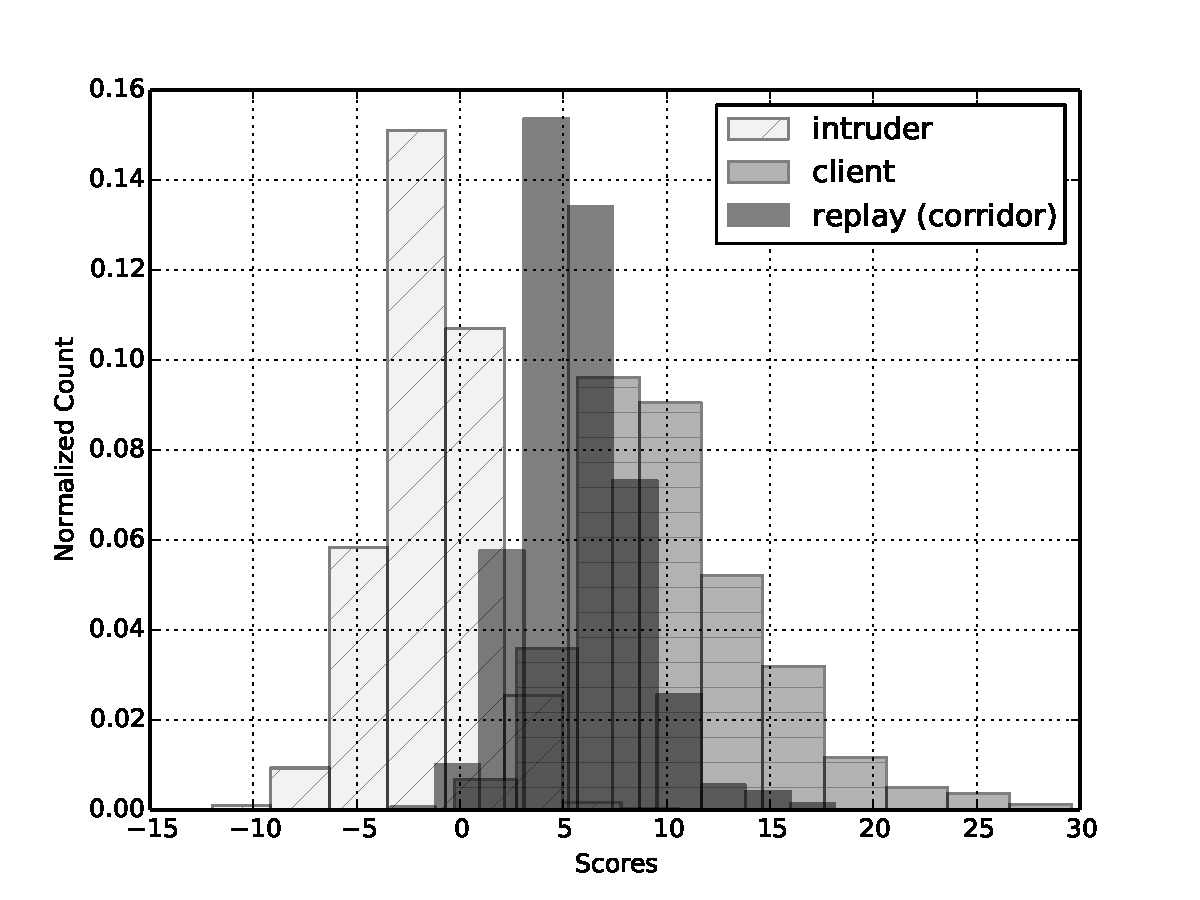
\includegraphics[width=1\linewidth]{Figs/dist_IV_corr.pdf}
%	\end{minipage}
%
%	\begin{minipage}{0.5\textwidth}
%	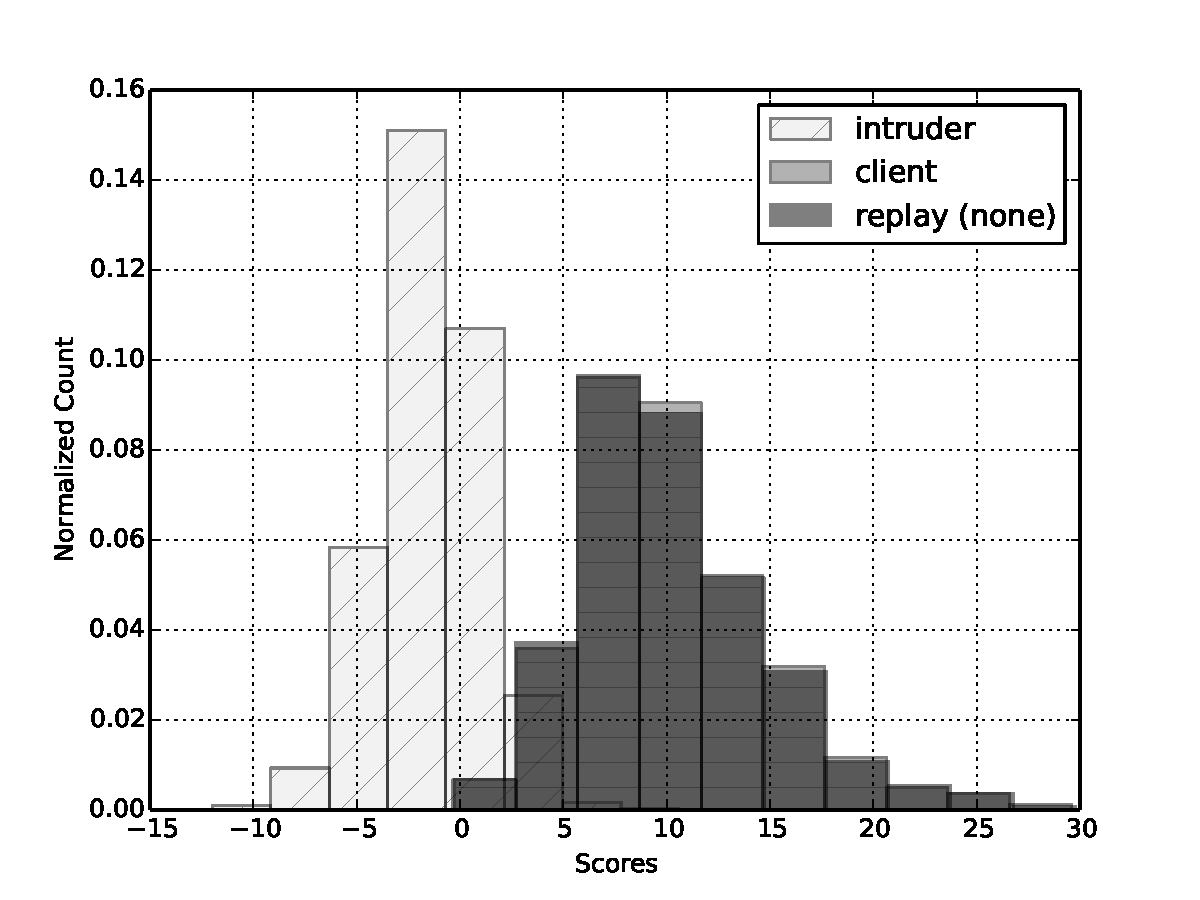
\includegraphics[width=1\linewidth]{Figs/dist_IV_none.pdf}
%	\end{minipage}

	\caption{Score distribution for the IV-PLDA system for replay attacks using a stand-alone speaker and emulation of an office.}
	\label{fig::Dist_IV}
\end{figure}

%DETs described
Fig.~\ref{fig::DETs_replay_GMM} and Fig.~\ref{fig::DETs_replay_IV} present the detection error trade-off (DET) plots\footnote{Produced with the TABULA RASA Scoretoolkit (http://publications.idiap.ch/downolads/reports/2012/Anjos\_Idiap-Com-02-2012.pdf)}  for the basic GMM-UBM and the state-of-the-art IV-PLDA systems, exposed to various replay attacks. They show that all replay attacks caused a significant degradation of the ASV performance. However, there are major differences in ASV performance depending on acoustic environment. If the acoustic environment is omitted, the ASV system is almost ideally spoofed -- the DET lines are close to straight, with the EER values close to 50\%. In realistic cases, when the room acoustics is taken into account, the spoofing is slightly less severe. It can be easily observed that the ASV performance under replay attack in a corridor is better than in an office, probably due to higher level of reverberation for the corridor. Fig.~\ref{fig::Dist_IV} shows a sample score distribution, here for the IV-PLDA system with a replay attack realised in an office (or with speech acquired in an office). A significant overlap of replay attacks with true client accesses can be observed.

In contrast, despite major differences in speakers' impulse responses (see Fig.~\ref{fig::IRs}), the differences between the DET plots corresponding to different speakers are only minor. It suggests a relatively low impact of a replay device on the effectiveness of replay attack. Since all seven ASV systems tested showed similar behaviour, therefore, for the sake of clearness, the next results will present the average of the three speakers used in experiments.


%EER table described
Table~\ref{tab::results_EER} shows the detailed EER results for replay attacks in various acoustic conditions against the seven various ASV systems, with and without score normalisation. All systems are shown to be severely sensitive to replay attacks. Even for the highly-reverberant corridor and the most resistant (in terms of EER) GSL kernel system with factor analysis and with T-norm, the EER rose to more than 22\% compared to the baseline 5.7\%. What was already visible in the DET plots (see Fig.~\ref{fig::DETs_replay_IV}), the results for the office are much worse -- the most resistant IV system (without PLDA and without score normalisation) and GSL-FA systems yielded the EER of ca. 28\%, whilst the other systems returned EERs of 30\% and more. If acoustic conditions are not emulated, the spoofing is almost perfect and the ASV systems yield EER values of 50\% or even more. 

It is noteworthy that under replay attack the iVector system with probabilistic linear discriminant analysis (PLDA) often shows worse results than the iVector system alone, even though the PLDA significantly decreases the EER for the baseline system (from 6.7\% down to less than 3\%, with score normalisation). This can be explained that in normal conditions the PLDA improves the performance of iVector-based ASV system as it compensates the intersession differences caused by channel or speaker variation. However, in the case of replay attack this can be disadvantageous, because it also seems to compensate the differences caused by replay devices and replay environments.

\begin{figure}
	\centering
	\begin{minipage}{.5\textwidth}
	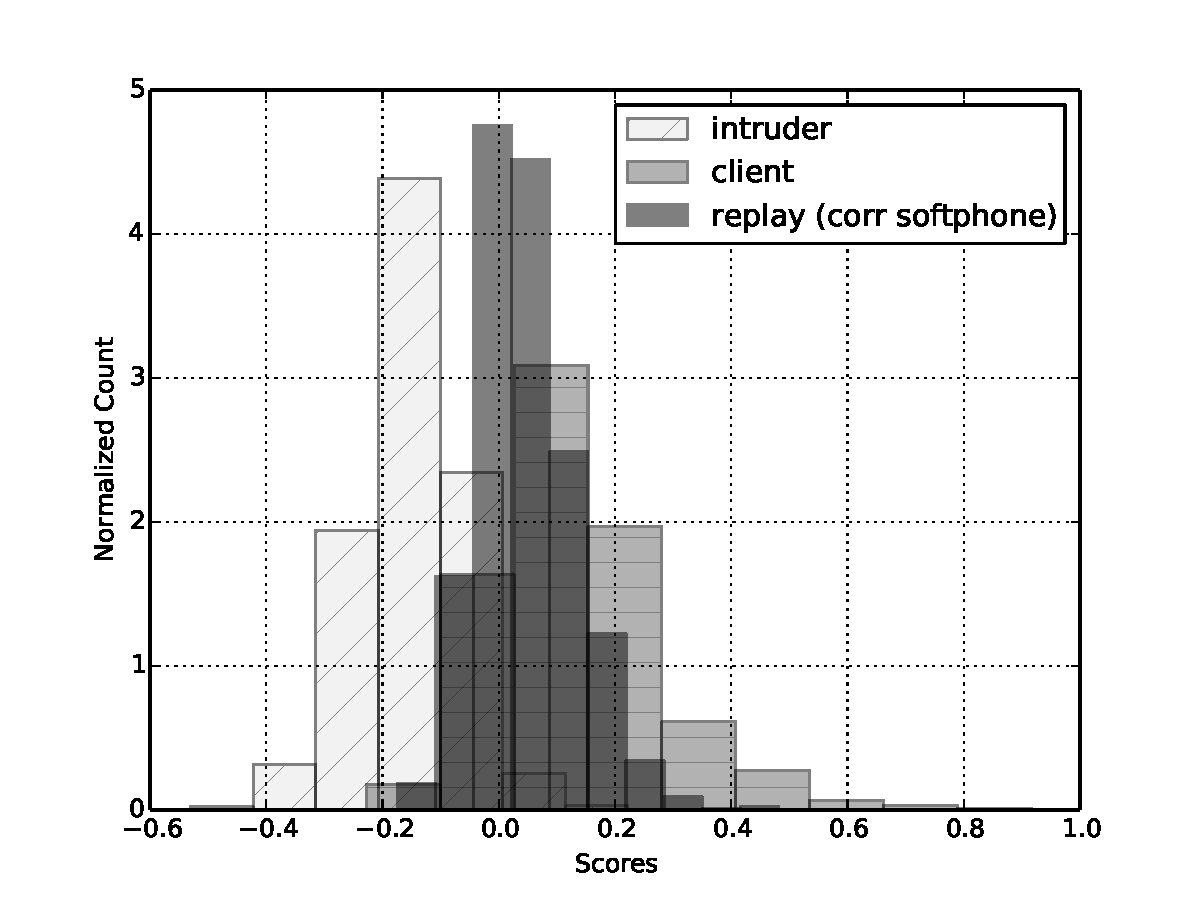
\includegraphics[width=1\linewidth]{Figs/dist_GMM_corr_iPhone.pdf}
%	\caption{DET plots for GMM-UBM (left) and i-Vectors-PLDA (right) systems.}
%	\label{fig::Dist_GMM_corr}
	\end{minipage}


	\begin{minipage}{0.5\textwidth}
	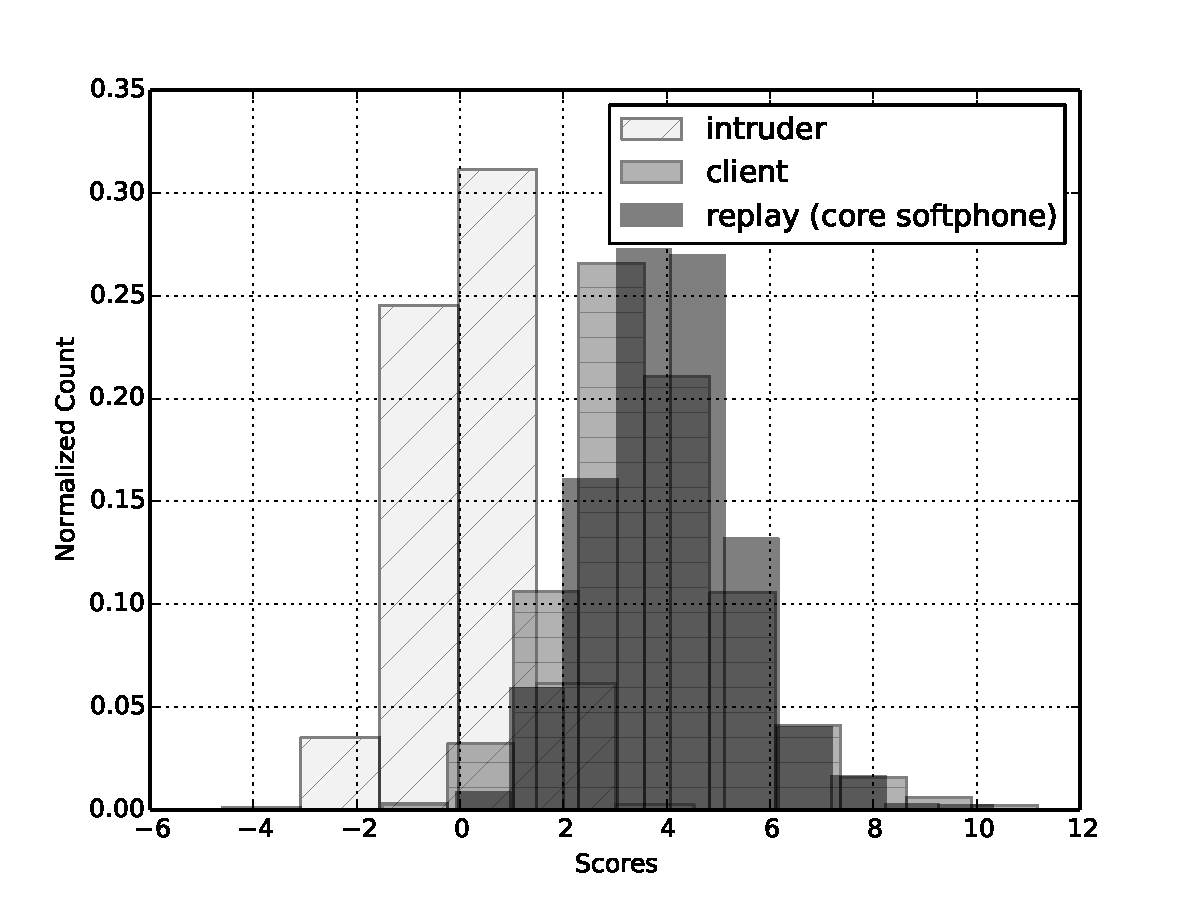
\includegraphics[width=1\linewidth]{Figs/dist_GMM_T_corr_iPhone.pdf}
%	\caption{DET plots for iVectors-PLDA xxxxxxxxxxxxxxxxxxx}
	\end{minipage}

	\caption{Score distribution for the GMM-UBM system without (top) and with (bottom) score normalisation.}
	\label{fig::Dist_GMM.T_corr}

\end{figure}



%% comparison with other attacks
\subsection{Comparison of replay threat vs. other spoofing methods}

\begin{table*}
%\ninept
\begin{center}
    \begin{tabular}{ l || c c c c c c}
    \hline
     	 Attack & GMM & SGL & SGL-NAP & SGL-FA & FA & IV-PLDA \\ 

 \hline \hline
Na\"{i}ve impostor & 9.08 & 7.89 & 6.35 & 6.08 & 5.60 & 3.20\\ 
Replay & 37.99	& 31.33 & 31.03 & 28.24 & 31.89 & 25.95\\
Voice conversion & 31.48 & 36.94 & 30.44 & 30.23 & 23.16 & 20.45\\ 
Speech synthesis & 39.90 & 14.66 & 13.83 & 11.98 & 30.81 & 10.92\\ 
\hline
    \end{tabular}
    \caption{EER values for different ASV systems for various spoofing attacks, without score normalisation.}
		\label{tab::results_EER_4attacks}
   \end{center}
\end{table*}


\begin{figure}
	\centering
	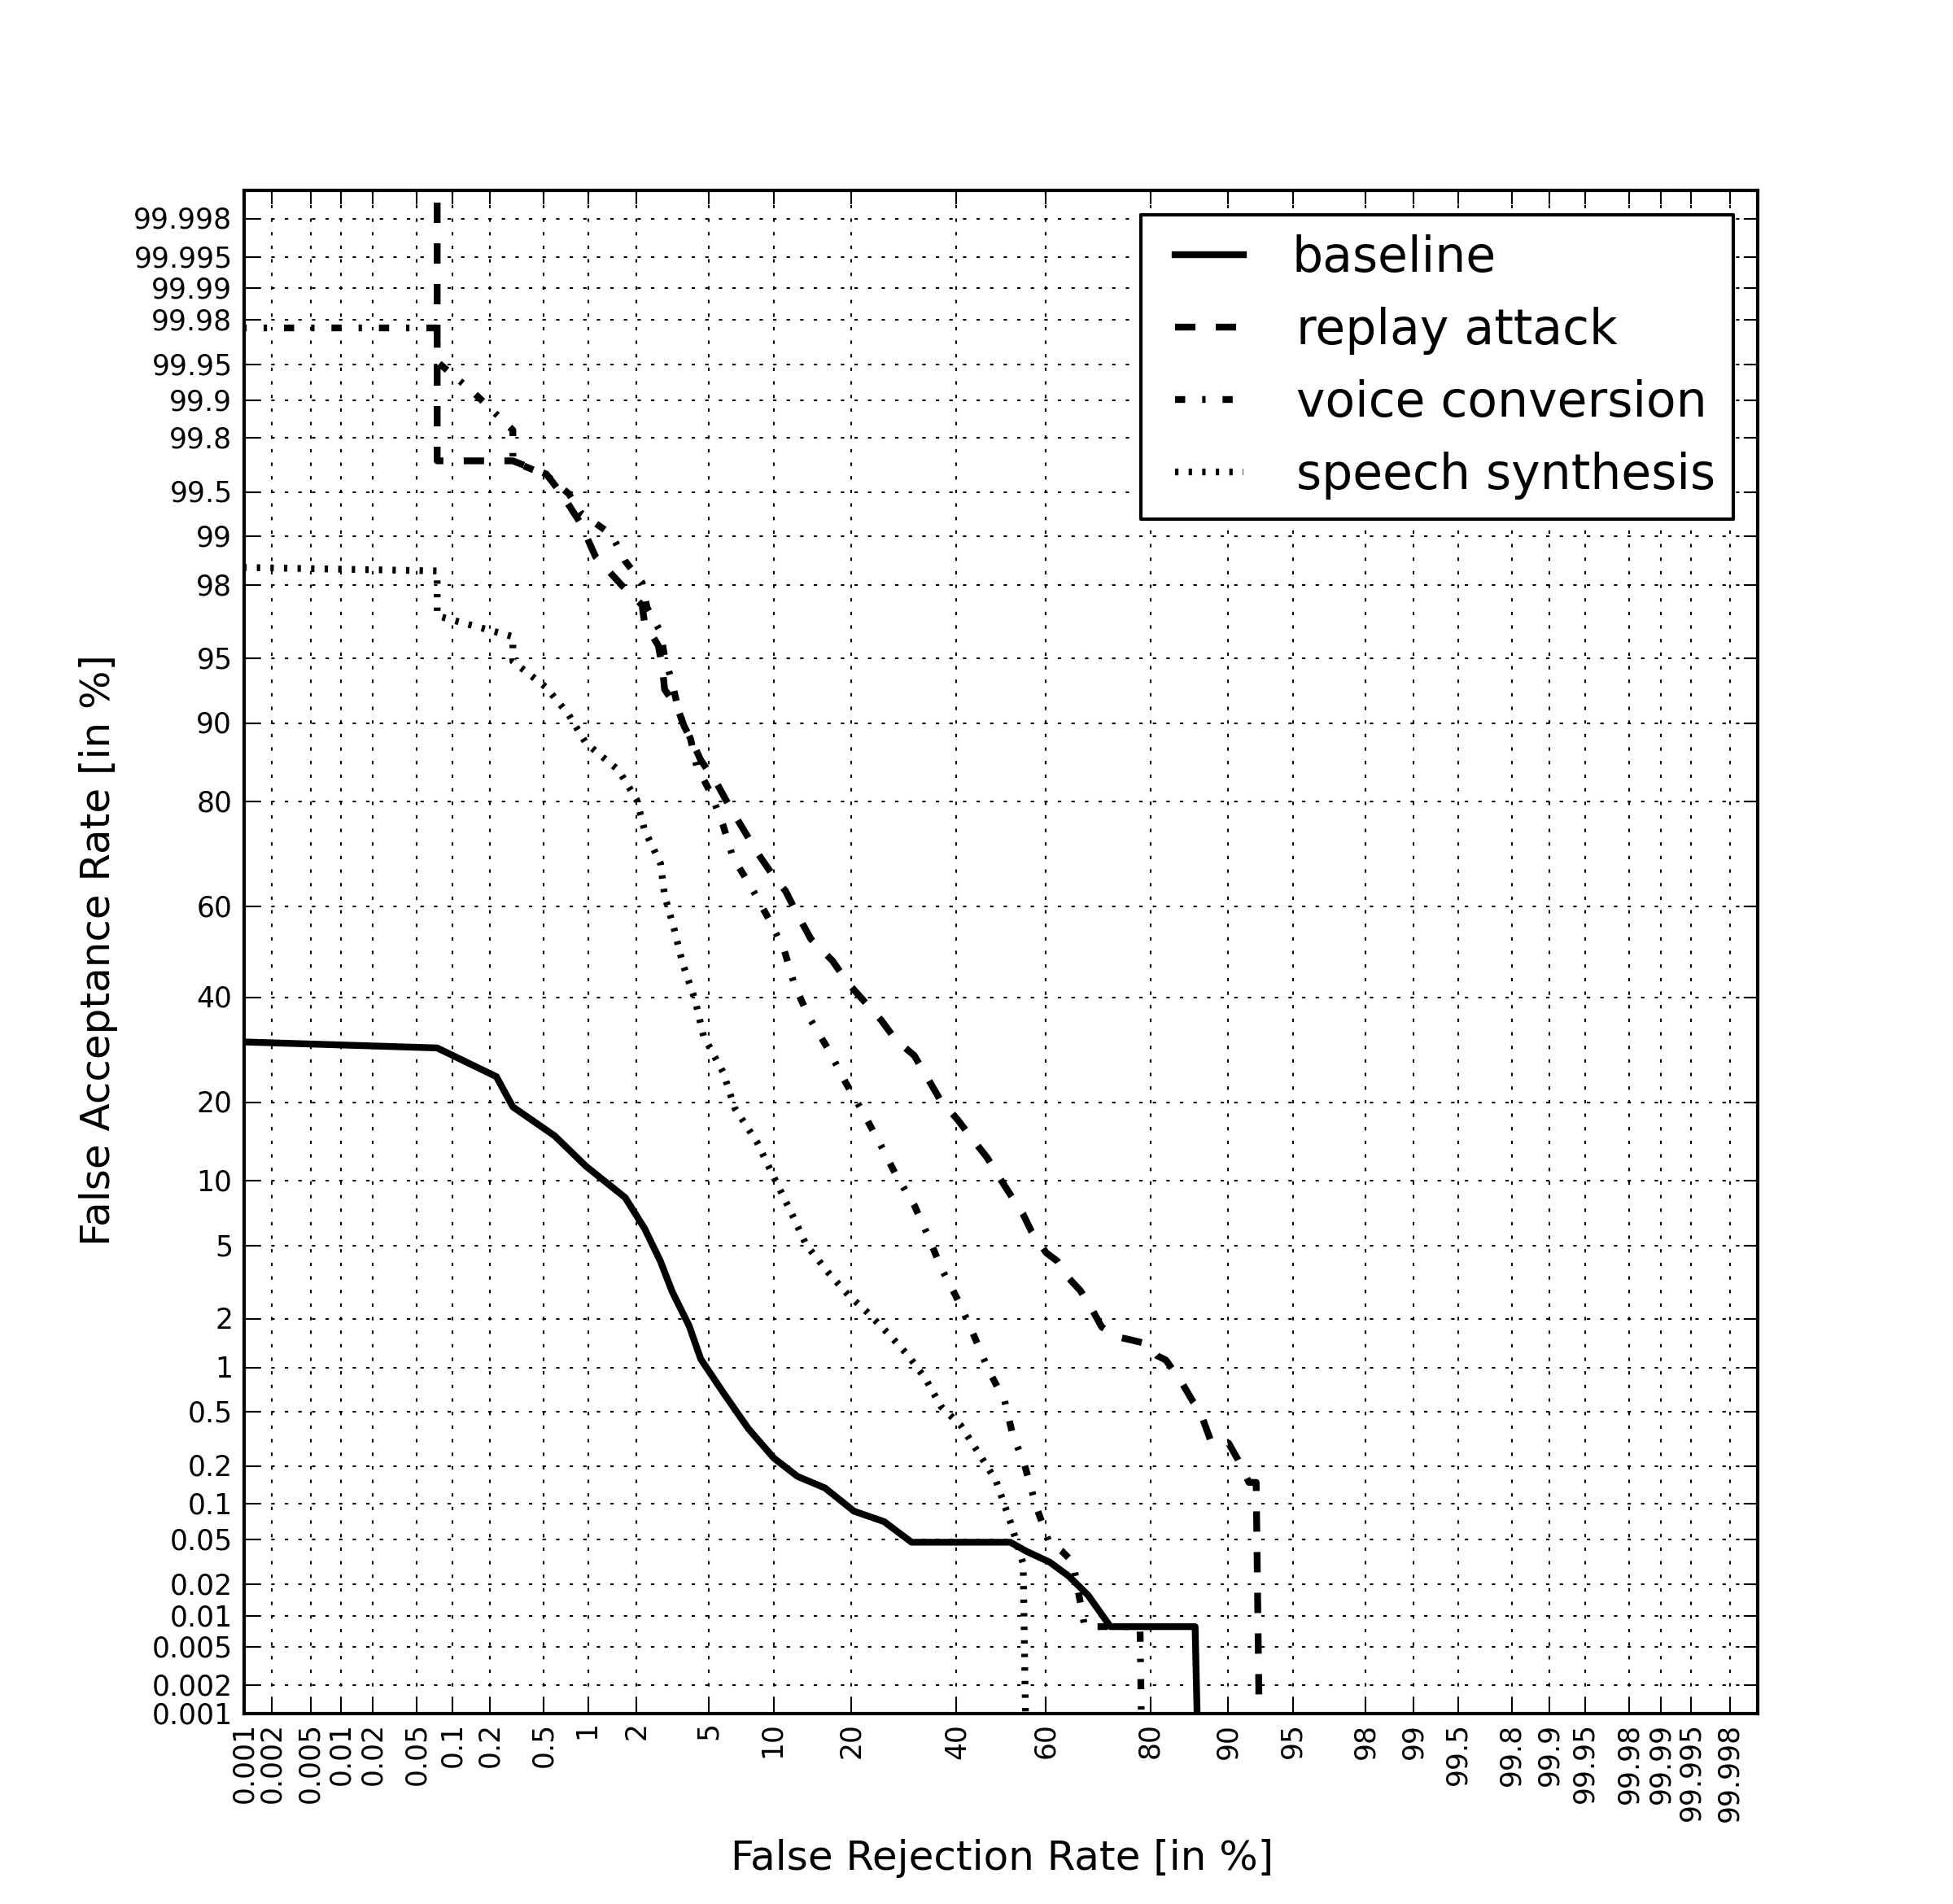
\includegraphics[width=1\linewidth]{Figs/DET_IV_ss_vc_rp.png}
	\caption{DET plots for iVector-PLDA system and various attacks.}
	\label{fig::DETs_4attacks}
\end{figure}

To compare the reply threat with the threat of voice conversion and speech synthesis, we took the average results for all replay devices, as well as the average for office and corridor as the replay environment.
The impact of voice conversion, despite demanding considerably more effort to implement, causes a similar degradation in performance to that of replay attacks. E.g., the SGL system yielded the EER of 37\% for voice conversion and on average 31\% for replay; in contrast, the IV-PLDA system showed to be more resistant to voice conversion than replay (20.5\% EER vs. 26\%, respectively). 

High-effort speech synthesis attacks proved much less effective -- the EER for the best IV-PLDA system reached less than 11\%, whilst replay attack caused an increase of the EER to 20.5\%. These observations are also illustrated through the DET plot in Fig.~\ref{fig::DETs_4attacks} for the IV-PLDA system.

%IN CONTRAST, it turns out that..... (REFERENCE TO BIOSIG PAPER ~\cite{Alegre2014}, SUMMARY OF THE RESULTS from THERE)
% displays... TBC.



\subsection{Impact of score normalisation}

The impact of score normalisation in the case of replay attack is ambiguous.  For some of the systems, such as factor analysis, GMM supervector linear kernel with factor analysis and with nuisance attribute projection the score normalisation helped to decrease EER values in the face of spoofing, e.g., for the factor analysis system and the corridor the EER decreased from almost 30\% to around 25\%. 

\begin{figure}
	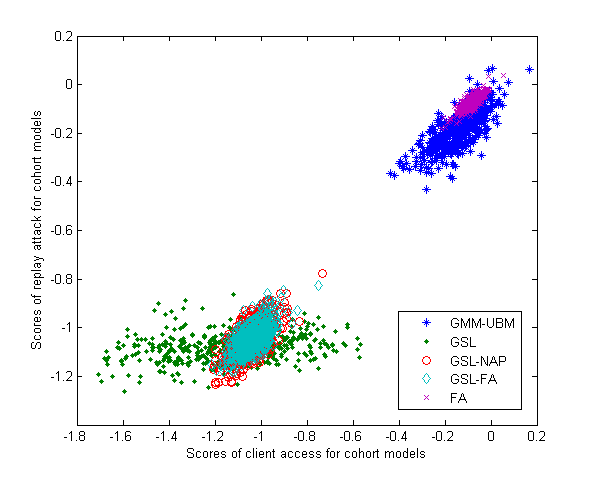
\includegraphics[width=1\linewidth]{Figs/Scores_cohort.png}

	\caption{Score distribution for replay attacks vs. client accesses calculated against cohort speaker models, for various ASVs.}
	\label{fig::Scores_cohort}
\end{figure}

In contrast, for four other ASV systems (GMM-UBM, GMM supervector linear kernel alone and both iVector systems), the score normalisation in fact helped the spoofer. The increase of EER after applying score normalisation for the GMM-UBM or SGL system is immense, e.g., for replay in an office and the GSL system, the EER increased from 34\% to 93\%. This effect is also well illustrated by score distributions presented in Fig. \ref{fig::Dist_GMM.T_corr}, using the example of replay played back from a smartphone in a corridor against a GMM-UBM system. It shows that the scores, having been normalised, got shifted even more to the right than original client accesses. 

This phenomenon seems to be a side-effect of T-norm algorithm, which involves dividing the scores by standard deviation of the scores reached for a cohort of reference speaker models. Table~\ref{tab::scores_cohort} displays standard deviation values for the client accesses and replay spoofed accesses. It shows that standard deviation for client accesses is by far the largest for the GMM supervector linear kernel system (0.25) and it is also relatively high for the GMM-UBM system (0.09). We believe that this is caused by lack of any compensation mechanism for channel and intersession variability, both in the GMM-UBM and the GSL systems. Higher standard deviation causes shifting the scores of the licit client accesses to the left on the score axis. Contrary, other ASVs cause much lower score dispersion (0.06 or less), what is also visible in Fig.~\ref{fig::Scores_cohort}. 

In contrast, standard deviation of scores for replay attacks is pretty low (0.07 or less, see Table~\ref{tab::scores_cohort}) -- this makes the normalised scores increase, so this is why they are shifted to the right in Fig.~\ref{fig::Dist_GMM.T_corr}, and this is why such systems are so vulnerable to replay attacks. This may pose a significant risk to those ASV systems facing a replay attack.

\begin{table}
%\ninept
\begin{center}
    \begin{tabular}{ l || c c c c c }
    \hline
     	 Scores/ASVs & GMM & GSL & GSL-NAP & GSL-FA & FA\\ 

 \hline \hline
Client accesses & 0.086 & 0.252 & 0.063 & 0.057 & 0.032\\
Replay attacks & 0.072 & 0.060 & 0.068 & 0.059 & 0.027\\
\hline
    \end{tabular}
    \caption{Standard deviation of client access scores calculated against cohort speaker models during score normalisation.}
		\label{tab::scores_cohort}
   \end{center}
\end{table}


%\subsection{Impact of using PLDA with iVector systems}
%
%When analysing operation of various ASV systems, we also compared the performance of both iVector systems used in experiments - with and without probabilistic linear discriminant analysis (PLDA). The results in Table~\ref{tab::results_EER}, confirmed by Fig.~\ref{fig::EER_PLDA}, clearly show that even though the PLDA significantly decreases the EER for the baseline system (from 6.7\% down to less than 3\%, with score normalisation), it mostly increases the EER when under replay attack. E.g., for an office and score normalisation the EER rose from less to 29\% to 30.3\%. 
%
%This behaviour of PLDA can be explained as follows: in normal conditions the PLDA improves significantly the performance of iVector-based ASV system as it compensates the intersession differences caused by channel or speaker variation. However, in the case of replay attack this can be disadvantageous, because it also seems to compensate the differences caused by replay devices and replay environments.
%
%% EER w/wo PLDA
%\begin{figure}
%	\centering
%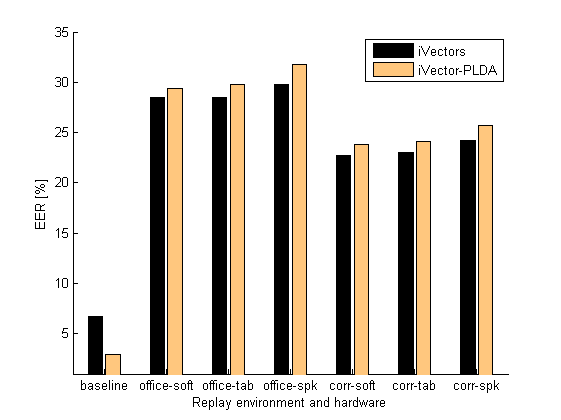
\includegraphics[width=1\linewidth]{Figs/EER_PLDA.png}
%	\caption{EER results for iVector-based ASV system with and without PLDA, with score normalisation used.}
%	\label{fig::EER_PLDA}
%\end{figure}


%\begin{figure}
%	\centering
%	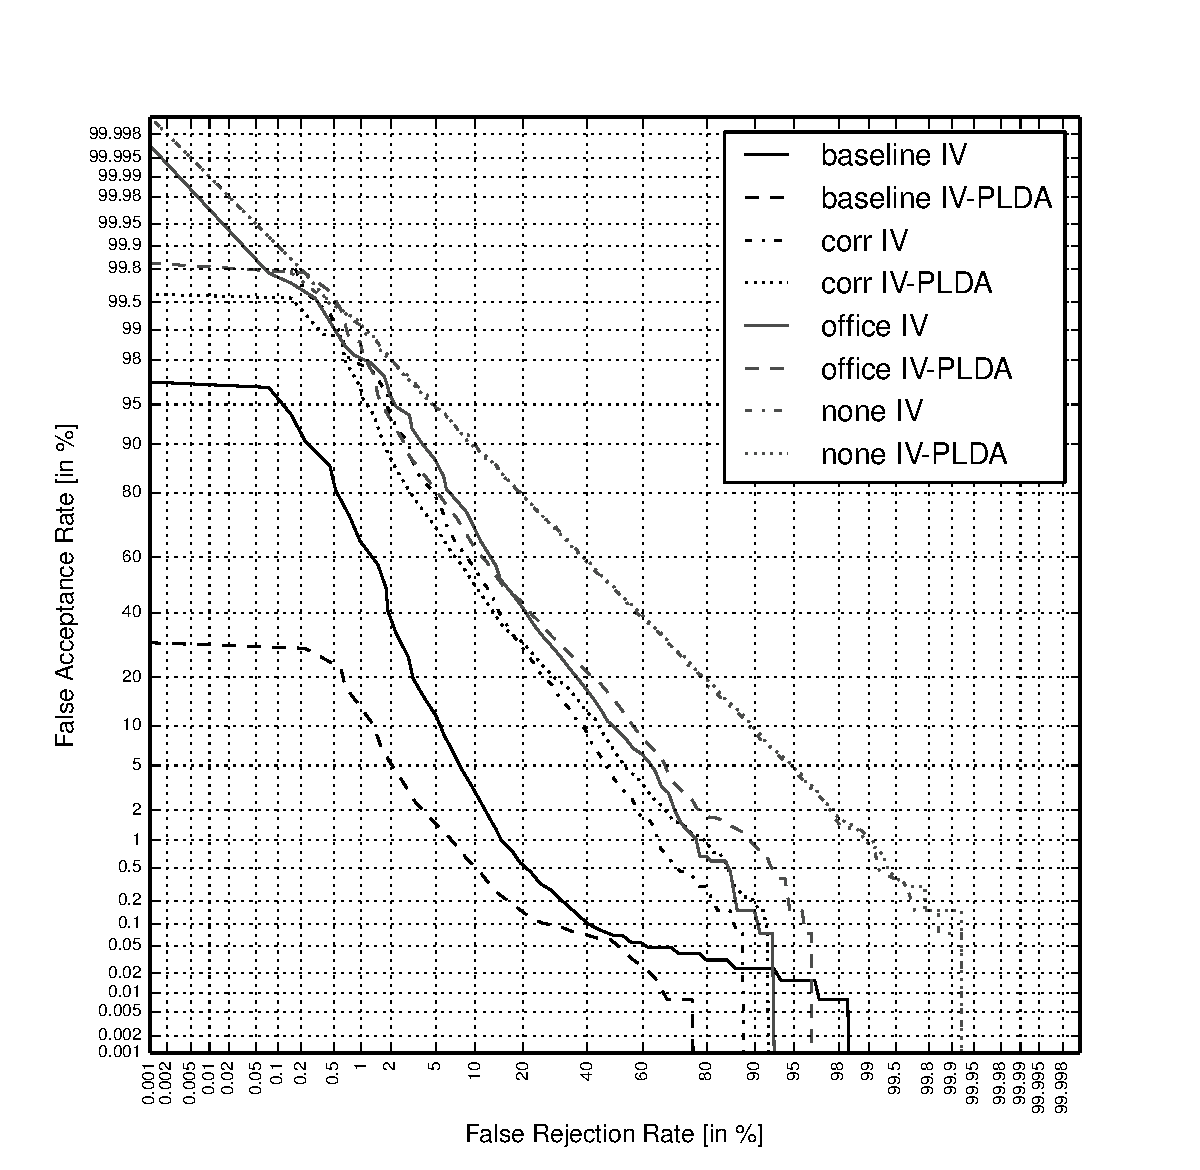
\includegraphics[width=1\linewidth]{Figs/DET_PLDA_iPad_Snorm.pdf}
%	\caption{DET plots for replay attack for the ASV based on iVectors with and without PLDA, with score normalisation (a tablet used as a replay device).}
%	\label{fig::DETs_PLDA}
%
%\end{figure}

\subsection{Results of experiments with the replay countermeasure}


\begin{table*}
%\ninept
\begin{center}
    \begin{tabular}{ l || c c c | c c c}
    \hline
 \multirow{2}{*}{Environment}  & \multicolumn{3}{c|}{EER (\%)} & \multicolumn{3}{c}{SFAR (\%)} \\
     	 & no CM & with FFD & with LBP & no CM & with FFD & with LBP\\ 

 \hline \hline
Office   & 30.30 & 13.62 & 9.56 & 88.70 & 63.93 & 46.29\\
Corridor & 24.53 & 11.34 & 7.00 & 80.91 & 50.25 & 30.52\\
None & 49.46 & 42.14 & 46.77 & 97.00 & 95.17 & 95.76\\
\hline
    \end{tabular}
    \caption{EER and SFAR values for various environment of replay attacks, with and without the FFD or LBP countermeasures applied, for IV-PLDA. The SFAR was measured for FRR equal to the baseline EER (2.98\%).}
		\label{tab::results_CM_rooms}
   \end{center}
\end{table*}


\begin{table*}
%\ninept
\begin{center}
    \begin{tabular}{ l || c c c | c c c}
    \hline
 \multirow{2}{*}{Environment}  & \multicolumn{3}{c|}{EER (\%)} & \multicolumn{3}{c}{SFAR (\%)} \\
     	 & no CM & with FFD & with LBP & no CM & with FFD & with LBP\\ 
 \hline \hline
Smartphone   & 33.96 & 11.66 & 7.52 & 88.38 & 54.83 & 36.79\\
Tablet & 34.48 & 11.82 & 7.50 & 88.42 & 55.33 & 36.83\\
Stand-alone speaker & 35.84 & 13.96 & 9.83 & 89.80 & 61.11 & 41.60\\
\hline
    \end{tabular}
    \caption{EER and SFAR values for various replay devices used for attacks, with and without the FFD or LBP countermeasures applied, for IV-PLDA. The SFAR was measured for FRR equal to the baseline EER (2.98\%).}
		\label{tab::results_CM_spk}
   \end{center}
\end{table*}


The detailed results of experiments with FFD and LBP countermeasures for various replay environment, averaged across the replay devices, are presented in Table~\ref{tab::results_CM_rooms}. It shows that the countermeasure performance varies depending on acoustic environment. The relative improvement caused by the countermeasures turned out to be the highest for the office -- in this case the EER decreased from 30\% down to less than 14\% for FFD and less than 10\% for LBP. Also for the corridor LBP turned out to be more effective than FFD -- 7\% EER vs. 11\%, respectively, also the SFAR result was much lower (30\% vs. 46\%). When acoustic conditions were not considered, both countermeasures performed poorly, with the EER results slightly better for FFD. This is also visualised by the shape of the DET plots presented in Fig~\ref{fig::DETs_CM}.

Table~\ref{tab::results_CM_spk} displays the results of the countermeasure experiments for various replay devices, averaged across different acoustic environments (only office and corridor were taken into account, as they are by far most realistic). Also here the LBP-based countermeasure yields better results than FFD. Both countermeasures helped most for a smartphone and a tablet (the EER values decreased to less than 12\% for FFD and to 7.5\% for LBP). The results for a stand-alone speaker are only slightly worse (14\% and 10\%, respectively), most likely due to higher quality of this device (see much better frequency response shown in Fig.~\ref{fig::IRs}). 


%% DETs w/wo CM
\begin{figure}
	\centering
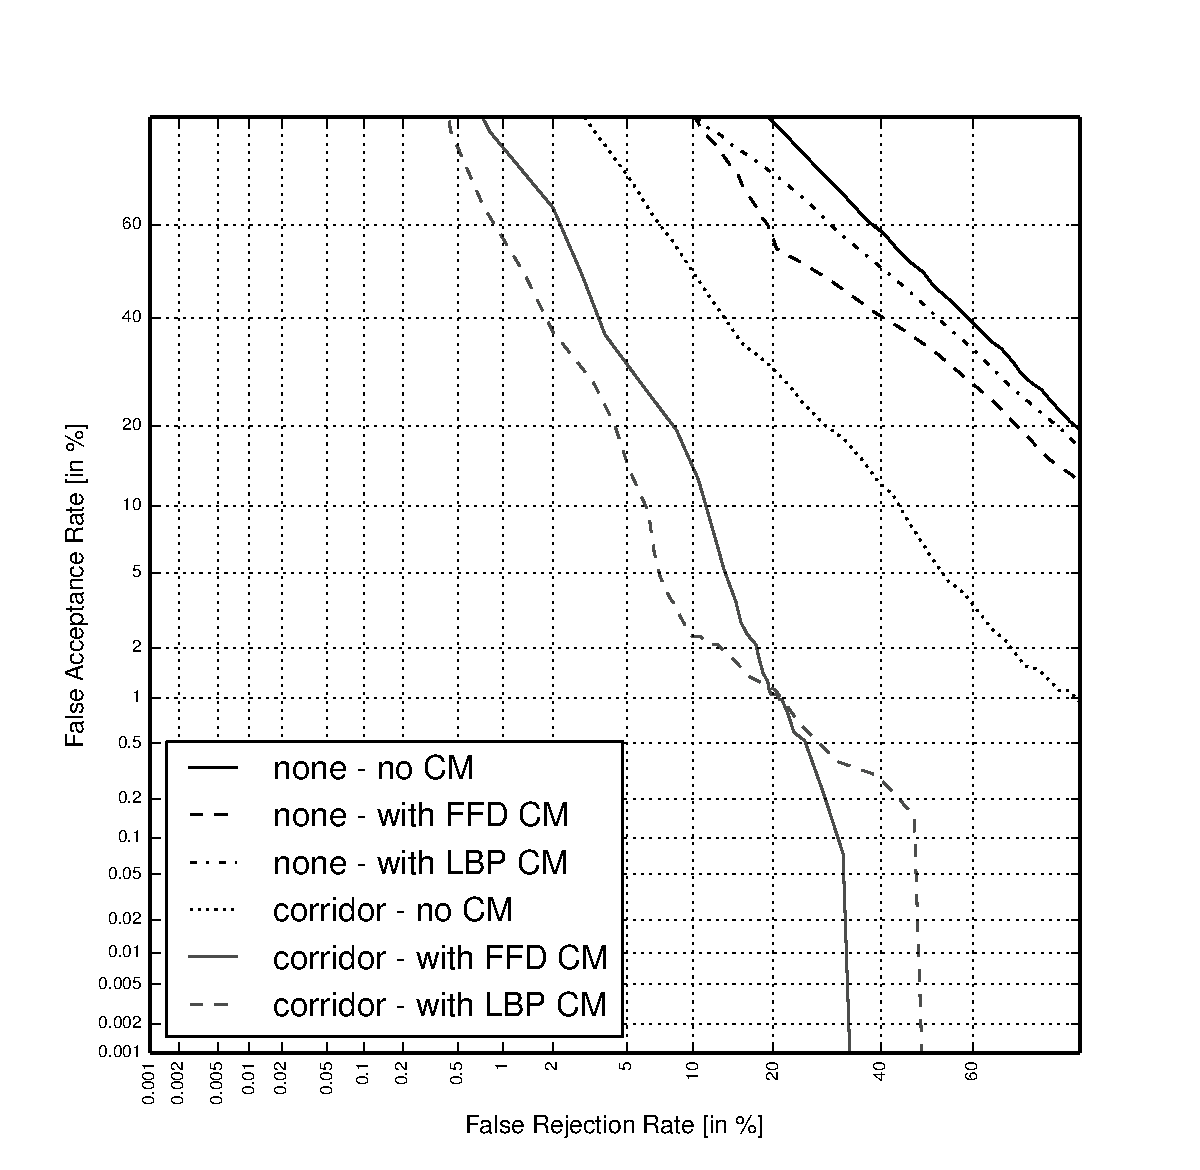
\includegraphics[width=1\linewidth]{Figs/DET_IVPLDA_counter_iPad.pdf}
	\caption{DET plots for IV-PLDA system for various replay environments, with and without the FFD or LBP countermeasures.}
	\label{fig::DETs_CM}
\end{figure}

